% questions.tex —— 2023 年·全国乙卷·文科 · 题目内容片段（无答案）
% 由 tools/generate_projects.py 依来源总账自 2023/2023_数学真题_全国乙文_试题.md 生成，勿手改（改源 MD 后重跑）


\par\medskip

\gkpart{一、单选题}

\begin{question}
\gkti{1}$|2+\mathrm i^2+2\mathrm i^3|=$\mbox{（　　）}

\begin{gkopts}(4)
\task A．$1$
\task B．$2$
\task C．$\sqrt5$
\task D．$5$
\end{gkopts}

\end{question}
\begin{question}
\gkti{2}设全集 $U=\{0,1,2,4,6,8\}$，集合 $M=\{0,4,6\}$，$N=\{0,1,6\}$，则 $M\cup\complement_U N=$\mbox{（　　）}

\begin{gkopts}(4)
\task A．$\{0,2,4,6,8\}$
\task B．$\{0,1,4,6,8\}$
\task C．$\{1,2,4,6,8\}$
\task D．$U$
\end{gkopts}

\Needspace{0.4\textheight}
\end{question}
\begin{question}
\gkti{3}如图，网格纸上绘制的是一个零件的三视图，网格小正方形的边长为 $1$，则该零件的表面积为\mbox{（　　）}
\nopagebreak[4]
\begin{center}\begin{tikzpicture}[x=0.42cm,y=0.42cm,line cap=round,line join=round]
  % 左上视图：6×5 网格；原卷粗线轮廓及横线
  \foreach \x in {0,...,6} {\draw[black!35,line width=0.25pt] (\x,0)--(\x,5);}
  \foreach \y in {0,...,5} {\draw[black!35,line width=0.25pt] (0,\y)--(6,\y);}
  \draw[line width=0.85pt] (2,1) rectangle (4,4);
  \draw[line width=0.85pt] (2,3)--(4,3);

  % 右上视图：6×5 网格；两级台阶轮廓
  \begin{scope}[xshift=7cm]
    \foreach \x in {0,...,6} {\draw[black!35,line width=0.25pt] (\x,0)--(\x,5);}
    \foreach \y in {0,...,5} {\draw[black!35,line width=0.25pt] (0,\y)--(6,\y);}
    \draw[line width=0.85pt] (2,1)--(3,1)--(3,2)--(4,2)--(4,4)--(2,4)--cycle;
  \end{scope}

  % 下方视图：6×5 网格；2×2 粗线矩形
  \begin{scope}[yshift=-6cm]
    \foreach \x in {0,...,6} {\draw[black!35,line width=0.25pt] (\x,0)--(\x,5);}
    \foreach \y in {0,...,5} {\draw[black!35,line width=0.25pt] (0,\y)--(6,\y);}
    \draw[line width=0.85pt] (2,1) rectangle (4,3);
  \end{scope}
\end{tikzpicture}
\end{center}
\nopagebreak[4]
\begin{gkopts}(4)
\task A．$24$
\task B．$26$
\task C．$28$
\task D．$30$
\end{gkopts}

\end{question}
\begin{question}
\gkti{4}记 $\triangle ABC$ 的内角 $A$，$B$，$C$ 的对边分别为 $a$，$b$，$c$，若 $a\cos B-b\cos A=c$，且 $C=\dfrac\pi5$，则 $B=$\mbox{（　　）}

\begin{gkopts}(2)
\task A．$\dfrac\pi{10}$
\task B．$\dfrac\pi5$
\task C．$\dfrac{3\pi}{10}$
\task D．$\dfrac{2\pi}5$
\end{gkopts}

\end{question}
\begin{question}
\gkti{5}已知 $f(x)=\dfrac{xe^x}{e^{ax}-1}$ 是偶函数，则 $a=$\mbox{（　　）}

\begin{gkopts}(4)
\task A．$-2$
\task B．$-1$
\task C．$1$
\task D．$2$
\end{gkopts}

\end{question}
\begin{question}
\gkti{6}已知正方形 $ABCD$ 的边长为 $2$，$E$ 为 $AB$ 的中点，则 $\overrightarrow{EC}\cdot\overrightarrow{ED}=$\mbox{（　　）}

\begin{gkopts}(4)
\task A．$\sqrt5$
\task B．$3$
\task C．$2\sqrt5$
\task D．$5$
\end{gkopts}

\end{question}
\begin{question}
\gkti{7}设 $O$ 为平面直角坐标系的坐标原点，在区域 $\{(x,y)\mid 1\leqslant x^2+y^2\leqslant4\}$ 内随机取一点，记该点为 $A$，则直线 $OA$ 的倾斜角不大于 $\dfrac\pi4$ 的概率为\mbox{（　　）}

\begin{gkopts}(4)
\task A．$\dfrac18$
\task B．$\dfrac16$
\task C．$\dfrac14$
\task D．$\dfrac12$
\end{gkopts}

\end{question}
\begin{question}
\gkti{8}若函数 $f(x)=x^3+ax+2$ 存在 $3$ 个零点，则 $a$ 的取值范围是\mbox{（　　）}

\begin{gkopts}(4)
\task A．$(-\infty,-2)$
\task B．$(-\infty,-3)$
\task C．$(-4,-1)$
\task D．$(-3,0)$
\end{gkopts}

\end{question}
\begin{question}
\gkti{9}某学校举办作文比赛，共设 $6$ 个主题，每位参赛同学从中随机抽取一个主题准备作文．则甲、乙两位参赛同学抽到不同主题的概率为\mbox{（　　）}

\begin{gkopts}(4)
\task A．$\dfrac56$
\task B．$\dfrac23$
\task C．$\dfrac12$
\task D．$\dfrac13$
\end{gkopts}

\end{question}
\begin{question}
\gkti{10}已知函数 $f(x)=\sin(\omega x+\varphi)$ 在区间 $\left(\dfrac\pi6,\dfrac{2\pi}3\right)$ 单调递增，直线 $x=\dfrac\pi6$ 和 $x=\dfrac{2\pi}3$ 为函数 $y=f(x)$ 的图象的两条对称轴，则 $f\left(-\dfrac{5\pi}{12}\right)=$\mbox{（　　）}

\begin{gkopts}(2)
\task A．$-\dfrac{\sqrt3}{2}$
\task B．$-\dfrac12$
\task C．$\dfrac12$
\task D．$\dfrac{\sqrt3}{2}$
\end{gkopts}

\end{question}
\begin{question}
\gkti{11}已知 $x,y$ 满足 $x^2+y^2-4x-2y-4=0$，则 $x-y$ 的最大值是\mbox{（　　）}

\begin{gkopts}(2)
\task A．$1+\dfrac{3\sqrt2}{2}$
\task B．$4$
\task C．$1+3\sqrt2$
\task D．$7$
\end{gkopts}

\end{question}
\begin{question}
\gkti{12}设 $A,B$ 为双曲线 $x^2-\dfrac{y^2}{9}=1$ 上两点，下列四个点中，可以为线段 $AB$ 中点的是\mbox{（　　）}

\begin{gkopts}(4)
\task A．$(1,1)$
\task B．$(-1,2)$
\task C．$(1,3)$
\task D．$(-1,-4)$
\end{gkopts}

\end{question}
\gkpart{二、填空题}

\begin{question}
\gkti{13}已知点 $A(1,\sqrt5)$ 在抛物线 $C:y^2=2px$ 上，则 $A$ 到 $C$ 的准线的距离为 \gkblank{}．

\end{question}
\begin{question}
\gkti{14}若 $\theta\in\left(0,\dfrac\pi2\right)$，$\tan\theta=\dfrac13$，则 $\sin\theta-\cos\theta=$ \gkblank{}．

\end{question}
\begin{question}
\gkti{15}若 $x,y$ 满足约束条件

\nopagebreak[4]
\[
\begin{cases}
x-3y\leqslant-1,\\
x+2y\leqslant9,\\
3x+y\geqslant7,
\end{cases}
\]

则 $z=2x-y$ 的最大值为 \gkblank{}．

\end{question}
\begin{question}
\gkti{16}已知点 $S,A,B,C$ 均在半径为 $2$ 的球面上，$\triangle ABC$ 是边长为 $3$ 的等边三角形，$SA\perp$ 平面 $ABC$，则 $SA=$ \gkblank{}．

\end{question}
\gkpart{三、解答题}

\begin{question}
\gkti{17}某厂为比较甲、乙两种工艺对橡胶产品伸缩率的处理效应，进行 $10$ 次配对试验，每次配对试验选用材质相同的两个橡胶产品，随机地选其中一个用甲工艺处理，另一个用乙工艺处理，测量处理后的橡胶产品的伸缩率．甲、乙两种工艺处理后的橡胶产品的伸缩率分别记为 $x_i,y_i$（$i=1,2,\cdots,10$）．试验结果如下：

\begin{center}
\begingroup\setlength{\tabcolsep}{4pt}
\begin{tabular}{crrrrrrrrrr}
\toprule
试验序号 $i$ & 1 & 2 & 3 & 4 & 5 & 6 & 7 & 8 & 9 & 10 \\
\midrule
伸缩率 $x_i$ & 545 & 533 & 551 & 522 & 575 & 544 & 541 & 568 & 596 & 548 \\
伸缩率 $y_i$ & 536 & 527 & 543 & 530 & 560 & 533 & 522 & 550 & 576 & 536 \\
\bottomrule
\end{tabular}
\endgroup
\end{center}

记 $z_i=x_i-y_i$（$i=1,2,\cdots,10$），记 $z_1,z_2,\cdots,z_{10}$ 的样本平均数为 $\bar z$，样本方差为 $s^2$．

（1） 求 $\bar z,s^2$；

（2） 判断甲工艺处理后的橡胶产品的伸缩率较乙工艺处理后的橡胶产品的伸缩率是否有显著提高（如果 $\bar z\geqslant2\sqrt{\dfrac{s^2}{10}}$，则认为甲工艺处理后的橡胶产品的伸缩率较乙工艺处理后的橡胶产品的伸缩率有显著提高，否则不认为有显著提高）．

\end{question}
\begin{question}
\gkti{18}记 $S_n$ 为等差数列 $\{a_n\}$ 的前 $n$ 项和．已知 $a_2=11$，$S_{10}=40$．

（1） 求 $\{a_n\}$ 的通项公式；

（2） 求数列 $\{|a_n|\}$ 的前 $n$ 项和 $T_n$．

\Needspace{0.4\textheight}
\end{question}
\begin{question}
\gkti{19}如图，在三棱锥 $P-ABC$ 中，$AB\perp BC$，$AB=2$，$BC=2\sqrt2$，$PB=PC=\sqrt6$，$BP,AP,BC$ 的中点分别为 $D,E,O$，点 $F$ 在 $AC$ 上，$BF\perp AO$．
\nopagebreak[4]
\begin{center}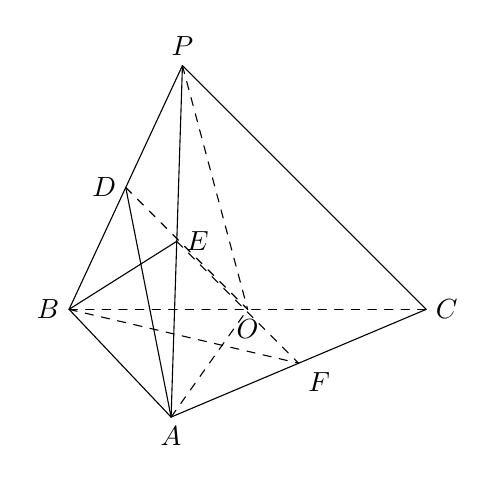
\begin{tikzpicture}[x=0.72cm,y=0.72cm,line cap=round,line join=round]
  \coordinate (P) at (2.0,6.6);
  \coordinate (A) at (1.8,0.4);
  \coordinate (B) at (0,2.3);
  \coordinate (C) at (6.3,2.3);
  \coordinate (D) at (1.0,4.45);
  \coordinate (E) at (1.9,3.5);
  \coordinate (O) at (3.15,2.3);
  \coordinate (F) at (4.05,1.35);

  % 三棱锥外棱及面内可见线
  \draw (P)--(B)--(A)--(C)--(P);
  \draw (P)--(A);
  \draw (D)--(A);
  \draw (B)--(E);
  \draw[dashed] (E)--(F);

  % 原图中的遮挡线
  \draw[dashed] (B)--(C);
  \draw[dashed] (P)--(O);
  \draw[dashed] (D)--(O);
  \draw[dashed] (A)--(O);
  \draw[dashed] (B)--(F);

  \node[above] at (P) {$P$};
  \node[below] at (A) {$A$};
  \node[left] at (B) {$B$};
  \node[right] at (C) {$C$};
  \node[left] at (D) {$D$};
  \node[right] at (E) {$E$};
  \node[below] at (O) {$O$};
  \node[below right] at (F) {$F$};
\end{tikzpicture}
\end{center}
\nopagebreak[4]
（1） 证明：$EF\parallel$ 平面 $ADO$；

（2） 若 $\angle POF=120^\circ$，求三棱锥 $P-ABC$ 的体积．

\end{question}
\begin{question}
\gkti{20}已知函数 $f(x)=\left(\dfrac1x+a\right)\ln(1+x)$．

（1） 当 $a=-1$ 时，求曲线 $y=f(x)$ 在点 $(1,f(1))$ 处的切线方程；

（2） 若 $f(x)$ 在 $(0,+\infty)$ 单调递增，求 $a$ 的取值范围．

\end{question}
\begin{question}
\gkti{21}已知椭圆 $C:\dfrac{y^2}{a^2}+\dfrac{x^2}{b^2}=1$（$a>b>0$）的离心率为 $\dfrac{\sqrt5}{3}$，点 $A(-2,0)$ 在 $C$ 上．

（1） 求 $C$ 的方程；

（2） 过点 $(-2,3)$ 的直线交 $C$ 于 $P,Q$ 两点，直线 $AP,AQ$ 与 $y$ 轴的交点分别为 $M,N$，证明：线段 $MN$ 的中点为定点．

\end{question}
\begin{question}
\gkti{22}在直角坐标系 $xOy$ 中，以坐标原点为极点，$x$ 轴正半轴为极轴建立极坐标系，曲线 $C_1$ 的极坐标方程为 $\rho=2\sin\theta\ \left(\dfrac\pi4\leqslant\theta\leqslant\dfrac\pi2\right)$．曲线 $C_2$：

\nopagebreak[4]
\[
\begin{cases}
x=2\cos\alpha,\\
y=2\sin\alpha,
\end{cases}
\qquad(\alpha\text{ \text{为参数，}}\ \dfrac\pi2<\alpha<\pi).
\]

（1） 写出 $C_1$ 的直角坐标方程；

（2） 若直线 $y=x+m$ 既与 $C_1$ 没有公共点，也与 $C_2$ 没有公共点，求 $m$ 的取值范围．

\end{question}
\begin{question}
\gkti{23}已知 $f(x)=2|x|+|x-2|$．

（1） 求不等式 $f(x)\leqslant6-x$ 的解集；

\Needspace{5\baselineskip}
（2） 在直角坐标系 $xOy$ 中，求不等式组

\nopagebreak[4]
\[
\begin{cases}
f(x)\leqslant y,\\
x+y-6\leqslant0
\end{cases}
\]

所确定的平面区域的面积．

\end{question}